\documentclass[11pt]{article}

\usepackage[margin=1in]{geometry}
\usepackage{amsmath}
\usepackage{amssymb}
\usepackage{graphicx}

% monospace \texttt tokens cannot hyphenate; let TeX stretch a line rather than overflow
\emergencystretch=1em

\title{705.641.81: Homework 3}
\author{David Carrillo}
\date{}

\begin{document}
\maketitle

\section{Concepts, intuitions and big picture}

\begin{enumerate}
  \item Weights and biases initialised to zero. True statements:
        \begin{itemize}
          \item[{[X]}] Each neuron in the first hidden layer will perform the same computation. So even
                after multiple iterations of gradient descent each neuron will be computing the same thing
                as other neurons in the same layer.
          \item[{[\ ]}] Each neuron in the first hidden layer will perform the same computation in the
                first iteration. But after one iteration of gradient descent they will learn to compute
                different things because we have ``broken symmetry''.
          \item[{[\ ]}] Each neuron in the first hidden layer will compute the same thing, but neurons in
                different layers will compute different things, thus we have accomplished ``symmetry
                breaking'' as described in lecture.
          \item[{[\ ]}] The first hidden layer's neurons will perform different computations from each
                other even in the first iteration; their parameters will thus keep evolving in their own way.
        \end{itemize}

  \item Vectorization allows forward propagation without an explicit loop over the layers
        $l = 1, 2, \ldots, L$.
        \begin{itemize}
          \item[{[\ ]}] True
          \item[{[X]}] False
        \end{itemize}

  \item \texttt{tanh} usually works better than sigmoid for hidden units because its output mean is closer
        to zero.
        \begin{itemize}
          \item[{[X]}] True
          \item[{[\ ]}] False
        \end{itemize}

  \item Which technique does NOT prevent overfitting?
        \begin{itemize}
          \item[{[\ ]}] Data augmentation \quad
          \item[{[\ ]}] Dropout \quad
          \item[{[\ ]}] Early stopping \quad
          \item[{[X]}] None of the above
        \end{itemize}

  \item During training, dropout zeroes a random subset of units on every step, so no single unit can
        be relied on and the network is forced to spread the same information across several units,
        which is what improves generalisation. At evaluation the goal is the opposite: a deterministic
        prediction that uses the whole network. Leaving dropout on would discard a random part of the
        model on every forward pass, so the same input would give different answers and the reported
        accuracy would carry avoidable variance. Turning it off and rescaling recovers the average
        behaviour the network was trained to produce.

  \item A constant initialisation makes every unit in a layer identical: they see the same input, compute
        the same output, and therefore receive the same gradient, so they perform the same update and stay
        identical forever. The layer then has the representational capacity of a single unit no matter how
        wide it is, and nothing in gradient descent can break the tie. Section 4 shows this concretely for
        XOR, where the all-zero case is even worse than a general constant because the hidden activations
        are exactly zero and the gradients with respect to $W_1$ and $W_2$ both vanish.

  \item No. Large positive weights make the pre-activations large in magnitude, which is exactly where the
        sigmoid saturates: its derivative is $\sigma(1-\sigma)$, which measures $2.5\times10^{-3}$ at $|z| = 6$ against a maximum of $0.25$ at $z = 0$. Gradients arriving at earlier layers are
        multiplied by one such factor per layer, so they vanish and those layers stop learning. Sigmoid is
        also not zero-centred, which compounds the problem described in item 3.

  \item A residual connection adds the block's input to its output, $h = x + F(x)$. Because the local
        derivative of a sum with respect to either input is the identity, the gradient reaching $x$ is the
        upstream gradient \emph{copied}, not attenuated, so there is always an unmultiplied path from the
        loss back to the early layers. That is what makes very deep stacks trainable, and it also means a
        block only has to learn the residual $F(x)$ rather than the whole mapping, so a block that learns
        nothing degrades to the identity instead of destroying the signal.

  \item What is cached (``memoized'') in forward and backward propagation?
        \begin{itemize}
          \item[{[X]}] Variables computed during forward propagation are cached and passed on to the
                corresponding backward propagation step to compute derivatives.
          \item[{[\ ]}] Caching is used to keep track of the hyperparameters that we are searching over, to
                speed up computation.
          \item[{[\ ]}] Caching is used to pass variables computed during backward propagation to the
                corresponding forward propagation step. It contains useful values for forward propagation
                to compute activations.
        \end{itemize}

  \item Which statement is true?
        \begin{itemize}
          \item[{[X]}] The deeper layers of a neural network are typically computing more complex features
                of the input than the earlier layers.
          \item[{[\ ]}] The earlier layers of a neural network are typically computing more complex
                features of the input than the deeper layers.
        \end{itemize}
\end{enumerate}

\section{Revisiting Jacobians}

Throughout, $X$ is $n \times d$ with rows $x_i \in \mathbb{R}^{d}$, $Y$ is $n \times k$, $W$ is
$k \times d$, and $w$ is $d \times 1$. The shape rule is
$\text{shape}(\mathbf{J}) = \text{shape(output)} \times \text{shape(input)}$, so differentiating by the
$d \times 1$ vector $w$ appends $d$ columns to whatever shape the output has.

\begin{enumerate}
  \item $f(w) = c$. The output is a scalar and the input is $d \times 1$, so the Jacobian is
        $1 \times d$. A constant does not depend on $w$, so every entry is zero:
        \[ \mathbf{J} = \mathbf{0}_{1 \times d}. \]

  \item $f(w) = \|w\|^2$. Scalar output, so $1 \times d$. Writing
        $\|w\|^2 = \sum_{i=1}^{d} w_i^2$, the $j$-th entry is
        $\partial/\partial w_j \sum_i w_i^2 = 2w_j$, and stacking into a row gives
        \[ \mathbf{J} = 2w^\top. \]

  \item $f(w) = w^\top x_i$. Scalar output, so $1 \times d$. With
        $w^\top x_i = \sum_{j} w_j x_{ij}$, the $j$-th entry is $x_{ij}$, so
        \[ \mathbf{J} = x_i^\top. \]

  \item $f(w) = Xw$. The output is $n \times 1$ and the input $d \times 1$, so the Jacobian is
        $n \times d$. The $i$-th output is $\sum_{j} X_{ij} w_j$, whose derivative with respect to
        $w_j$ is $X_{ij}$, which is the $(i,j)$ entry of $X$:
        \[ \mathbf{J} = X. \]

  \item $f(w) = w$. Output $d \times 1$, input $d \times 1$, so $d \times d$. Entry $(i,j)$ is
        $\partial w_i/\partial w_j = \delta_{ij}$:
        \[ \mathbf{J} = I_d. \]

  \item $f(w) = w^2$ elementwise. Output $d \times 1$, so $d \times d$. Entry $(i,j)$ is
        $\partial w_i^2/\partial w_j$, which is $2w_i$ when $i = j$ and zero otherwise, because output $i$
        depends only on input $i$:
        \[ \mathbf{J} = 2\,\mathrm{diag}(w). \]
        The off-diagonal zeros are the signature of an elementwise function.

  \item \textbf{Extra Credit.} $f(W) = XW^\top$. The output is $n \times k$ and the input is
        $k \times d$, so by the shape rule the Jacobian is a four-index tensor of shape
        $(n \times k) \times (k \times d)$, not a matrix. Taking a single entry,
        $(XW^\top)_{ia} = \sum_{c} X_{ic} W_{ac}$, and differentiating with respect to $W_{bc}$ leaves
        $X_{ic}$ only when $a = b$:
        \[ \mathbf{J}[i,a,b,c] = \frac{\partial (XW^\top)_{ia}}{\partial W_{bc}} = \delta_{ab}\, X_{ic}. \]
        So the tensor is block diagonal in the $(a,b)$ pair, with each diagonal block equal to $X$.
\end{enumerate}

Items 1 to 6 were checked against numerically computed Jacobians (central differences, $n=6$,
$d=4$, $k=3$), and item 7 against the full $6 \times 3 \times 3 \times 4$ numeric tensor; all agree
to within $10^{-4}$.

\section{Activations Per Layer, Keeps Linearity Away!}

\begin{enumerate}
  \item Without a non-linearity a stack of layers collapses: composing affine maps
        $W_2(W_1x + b_1) + b_2$ gives another affine map, so an arbitrarily deep network would represent
        exactly the same function class as a single linear layer and could only separate linearly separable
        data. The activation is what supplies representational capacity, which is why the universal
        approximation results are stated in terms of the non-linearity rather than the parameter count.

  \item The three functions and their derivatives:
        \[
          \sigma(z) = \frac{1}{1 + e^{-z}}, \qquad \sigma'(z) = \sigma(z)\big(1 - \sigma(z)\big)
        \]
        \[
          \tanh(z) = \frac{e^{z} - e^{-z}}{e^{z} + e^{-z}}, \qquad \tanh'(z) = 1 - \tanh^2(z)
        \]
        \[
          \mathrm{ReLU}(z) = \max(0, z), \qquad
          \mathrm{ReLU}'(z) = \begin{cases} 1 & z > 0 \\ 0 & z < 0 \end{cases}
          \quad \text{(undefined at } z = 0\text{)}
        \]
        \begin{center}
          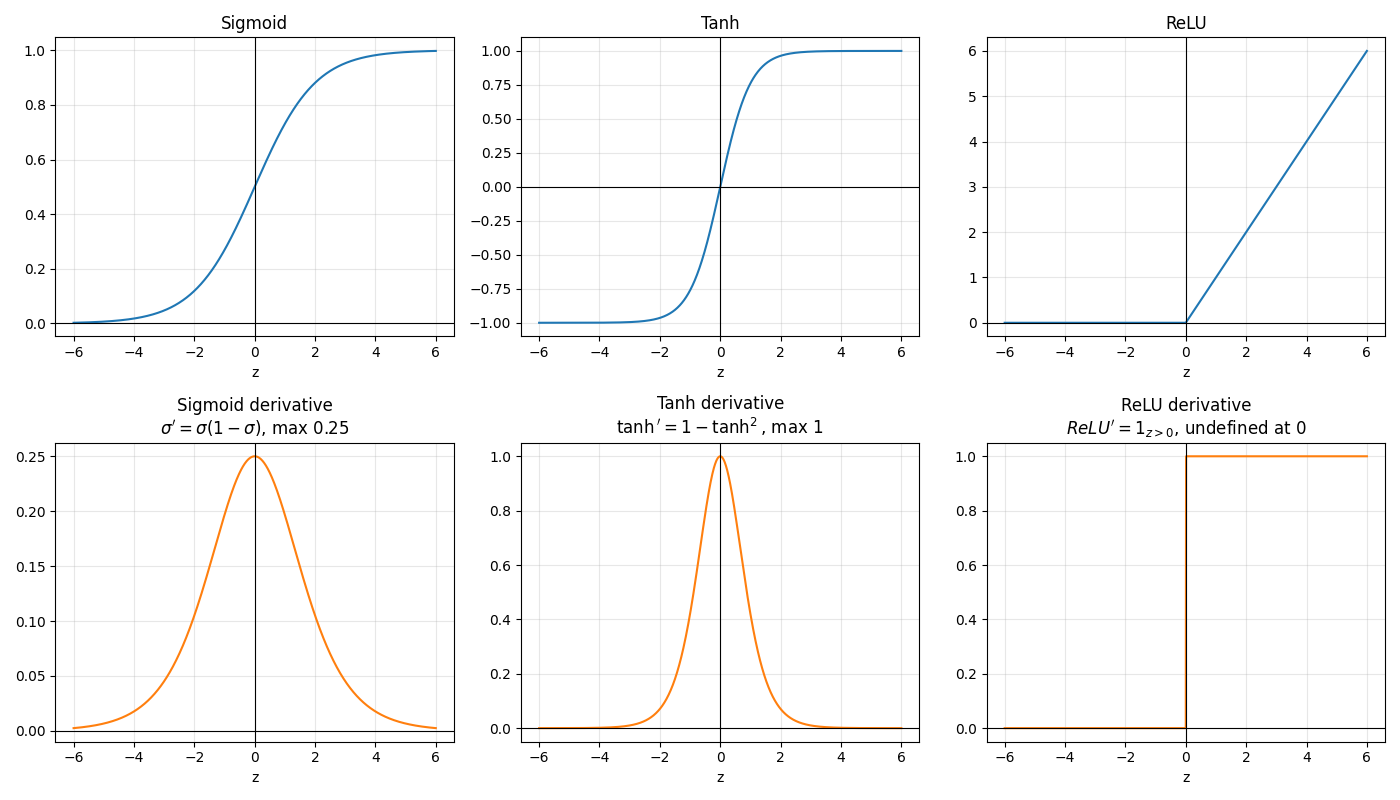
\includegraphics[width=0.9\textwidth]{hw3/activations.png}
        \end{center}

  \item The vanishing gradient problem is that backpropagation multiplies one activation derivative per
        layer, so when those derivatives are smaller than one the gradient reaching early layers shrinks
        exponentially in depth and those layers effectively stop learning. Sigmoid and \texttt{tanh} are
        both subject to it because they saturate: their derivatives go to zero for large $|z|$, which measure $2.5 \times 10^{-3}$ and $2.5\times10^{-5}$ respectively at $|z| = 6$. Sigmoid is worse
        even away from saturation, because its derivative never exceeds $0.25$, so the gradient shrinks by
        at least a factor of four per layer ($0.25^{10} \approx 10^{-6}$), whereas ReLU's derivative is
        exactly $1$ on the active side and does not attenuate at all.

  \item A layer's weight gradient is the outer product of the incoming error with that layer's input
        activations. If those activations are all non-negative, as with sigmoid (measured mean $+0.50$) or
        ReLU (measured mean $+1.50$), then every weight feeding a given unit has a gradient of the same
        sign on any single step, so the whole row can only move up together or down together. Updates then
        zig-zag toward the optimum instead of heading straight for it, which slows convergence. A
        zero-centred activation such as \texttt{tanh} (measured mean $0.00$) produces activations of both
        signs, so the weights in a row can move in different directions on the same step.

  \item Write $\sigma(\mathbf{z})_i = e^{z_i} / S$ with $S = \sum_{l=1}^{K} e^{z_l}$, and note
        $\partial S/\partial z_j = e^{z_j}$. By the quotient rule,
        \[
          \frac{d\sigma(\mathbf{z})_i}{dz_j}
          = \frac{\dfrac{\partial e^{z_i}}{\partial z_j}\, S - e^{z_i}\, \dfrac{\partial S}{\partial z_j}}{S^2}
          = \frac{\delta_{ij} e^{z_i} S - e^{z_i} e^{z_j}}{S^2}
          = \delta_{ij}\frac{e^{z_i}}{S} - \frac{e^{z_i}}{S}\frac{e^{z_j}}{S},
        \]
        where $\partial e^{z_i}/\partial z_j = \delta_{ij} e^{z_i}$ because $e^{z_i}$ depends on $z_j$ only
        when $i = j$. Substituting $\sigma(\mathbf{z})_i = e^{z_i}/S$ in both terms,
        \[
          \frac{d\sigma(\mathbf{z})_i}{dz_j}
          = \sigma(\mathbf{z})_i \delta_{ij} - \sigma(\mathbf{z})_i \sigma(\mathbf{z})_j
          = \sigma(\mathbf{z})_i\big(\delta_{ij} - \sigma(\mathbf{z})_j\big).
        \]

  \item The Jacobian collects those entries with $i$ indexing rows and $j$ columns, so
        $\mathbf{J}_\sigma(\mathbf{z})_{ij} = \sigma_i(\delta_{ij} - \sigma_j)$. Splitting the two terms,
        the $\delta_{ij}\sigma_i$ part is non-zero only on the diagonal and contributes
        $\mathrm{diag}(\sigma(\mathbf{z}))$, while the $-\sigma_i \sigma_j$ part is the $(i,j)$ entry of the
        outer product $-\sigma(\mathbf{z})\sigma(\mathbf{z})^\top$. Therefore
        \[
          \mathbf{J}_\sigma(\mathbf{z}) = \mathrm{diag}(\sigma(\mathbf{z}))
            - \sigma(\mathbf{z})\sigma(\mathbf{z})^\top \in \mathbb{R}^{K \times K}.
        \]
        Both inputs and outputs are $K$-vectors, which is why the shape is $K \times K$. Both forms were verified against central differences and against
        \texttt{torch.autograd.functional.jacobian} for $K = 5$.
        Two structural facts fall out and serve as a check: the matrix is symmetric, and its rows sum to
        zero, which they must because softmax outputs always sum to one so no perturbation of $\mathbf{z}$
        can change that total.
\end{enumerate}

\section{Simulating XOR}

\begin{enumerate}
  \item No. With $\hat{y} = \mathrm{ReLU}(W \cdot \mathbf{x} + b)$ the decision boundary is the single
        hyperplane $W \cdot \mathbf{x} + b = 0$, since ReLU is monotone and cannot change which side of
        that boundary a point falls on. XOR needs $(0,1)$ and $(1,0)$ to be positive while $(0,0)$ and
        $(1,1)$ are zero, and those two classes are not linearly separable: the positive pair and the
        negative pair each lie on a diagonal, so any line separating one diagonal cuts through the other.
        Concretely, a separating line would need $b < \tfrac{1}{2}$ from $(0,0)$, then
        $w_1 + b > \tfrac{1}{2}$ and $w_2 + b > \tfrac{1}{2}$ from the two positives, which forces
        $w_1 + w_2 + b > 1 - b > \tfrac{1}{2}$ and so makes $(1,1)$ positive too, contradicting the fourth
        requirement. A brute-force search over $41^3 = 68{,}921$ grid points for $(w_1, w_2, b)$ found zero
        solutions, as expected.

  \item A two-layer network does represent XOR. One set of weights that works exactly:
        \[
          W_1 = \begin{bmatrix} 1 & 1 \\ 1 & 1 \end{bmatrix}, \quad
          \mathbf{b}_1 = \begin{bmatrix} 0 \\ -1 \end{bmatrix}, \quad
          W_2 = \begin{bmatrix} 1 & -2 \end{bmatrix}, \quad
          b_2 = 0 .
        \]
        The two hidden units compute $\mathrm{ReLU}(x_1 + x_2)$ and $\mathrm{ReLU}(x_1 + x_2 - 1)$, that is
        ``at least one input is on'' and ``both inputs are on'', and the output subtracts twice the second
        from the first:
        \begin{center}
        \begin{tabular}{|c|c|c|}
          \hline
          $\mathbf{x}$ & $\mathbf{h} = \mathrm{ReLU}(W_1\mathbf{x} + \mathbf{b}_1)$ & $\hat{y} = W_2\mathbf{h} + b_2$ \\
          \hline
          $(0,0)$ & $[0, 0]$ & $0$ \\
          $(0,1)$ & $[1, 0]$ & $1$ \\
          $(1,0)$ & $[1, 0]$ & $1$ \\
          $(1,1)$ & $[2, 1]$ & $0$ \\
          \hline
        \end{tabular}
        \end{center}
        All four outputs match XOR exactly. The reason this works is that the hidden layer's ReLU bends
        the input space, so the output layer sees a representation in which the two classes \emph{are}
        linearly separable.

  \item With all weights and biases zero, the pre-activation is
        $W_1\mathbf{x} + \mathbf{b}_1 = \mathbf{0}$ for every input, so
        $\mathbf{h} = \mathrm{ReLU}(\mathbf{0}) = \mathbf{0}$ and $\hat{y} = b_2 = 0$ regardless of
        $\mathbf{x}$. Now consider the gradients. Writing $\ell' = \partial \ell / \partial \hat{y}$,
        \[
          \frac{\partial \ell}{\partial W_2} = \ell' \cdot \mathbf{h}^\top = \mathbf{0},
          \qquad
          \frac{\partial \ell}{\partial W_1}
            = \big(W_2^\top \ell' \odot \mathbf{1}[W_1\mathbf{x} + \mathbf{b}_1 > 0]\big)\mathbf{x}^\top
            = \mathbf{0},
        \]
        the first because $\mathbf{h} = \mathbf{0}$ and the second because $W_2 = \mathbf{0}$ (and the ReLU
        mask is zero as well). So both weight matrices have exactly zero gradient and never move; only
        $b_2$ receives a signal, and it can only learn the mean label. The network stays the constant
        function and can never represent XOR. Numerically, the gradient norms of $W_1$ and $W_2$ are
        exactly $0$ at every step and $W_1$ is still all zeros after training, while the loss converges to
        $0.25$, which is the variance of the XOR labels and exactly what the best constant predictor
        $b_2 = 0.5$ achieves.

  \item \textbf{Extra Credit.} Now let $\mathbf{h} = f(W_1\mathbf{x} + \mathbf{b}_1)$ for an arbitrary
        activation $f$, with every weight and bias initialised to the same constant $c$. Every row of
        $W_1$ is identical and every entry of $\mathbf{b}_1$ equals $c$, so all hidden pre-activations are
        the same number $c\left(\sum_j x_j\right) + c$ and every component of $\mathbf{h}$ is identical.

        The key point is that gradient descent cannot undo this. The gradient with respect to row $i$ of
        $W_1$ is
        \[
          \frac{\partial \ell}{\partial W_1^{(i)}}
            = \frac{\partial \ell}{\partial \hat{y}}\; W_{2}^{(i)}\; f'\big(c\textstyle\sum_j x_j + c\big)\;
              \mathbf{x}^\top ,
        \]
        and every factor on the right is the same for every $i$: the outgoing weights $W_2^{(i)}$ are all
        $c$, the pre-activation inside $f'$ is shared, and $\mathbf{x}$ is shared. Identical rows receiving
        identical gradients remain identical after any number of updates, and by the same argument all
        entries of $W_2$ stay equal to each other. So at every step the network computes
        \[
          \hat{y} = k\,w_2\, f\!\big(w_1 \textstyle\sum_j x_j + b_1\big) + b_2
        \]
        for scalars $w_1, w_2, b_1, b_2$ and hidden width $k$: it is permanently a \emph{single effective
        hidden unit}, no matter how wide the layer is. The solution in item 2 needs two hidden units that
        compute \emph{different} functions, and that region of parameter space is unreachable from a
        uniform initialisation.

        For any monotonic $f$ this settles it. A single effective unit gives an output that is a monotone
        function of $\sum_j x_j$, whereas XOR requires the non-monotone pattern $0, 1, 0$ as the sum goes
        $0, 1, 2$. Matching the two zeros would need $f(b_1) = f(2w_1 + b_1)$, which for strictly monotonic
        $f$ forces $w_1 = 0$ and then all three outputs coincide. Numerically, for $k = 4$ and $c = 0.5$, with sigmoid, \texttt{tanh} and ReLU the rows of $W_1$ are still identical after 300
        gradient descent steps at learning rate $0.5$ and the loss stalls at $0.21$, $0.25$ and $0.25$ respectively, ReLU
        degenerating to the constant $0.5$ on all four inputs.

        Worth stating precisely, since the question says \emph{arbitrary} $f$: the symmetry argument above
        holds for every $f$, but the final step uses monotonicity. A deliberately non-monotonic activation
        such as $f(u) = -(u-1)^2$ lets even one effective unit fit XOR, and in that case the collapsed
        network does reach a low loss. Every activation used in practice is monotonic, so the intended
        conclusion stands, but it is the monotonicity rather than the symmetry that rules XOR out.
\end{enumerate}

\section{Neural Nets and Backpropagation}

\begin{enumerate}
  \item Computation graph for $f(x,y,z) = \ln x + \exp(y)\cdot z$, one elementary operation per node:
        \[
          h_1 = \ln x, \qquad h_2 = \exp(y), \qquad h_3 = h_2 \cdot z, \qquad f = h_1 + h_3 .
        \]
        As a graph, $x \to h_1$, $y \to h_2$, then $h_2$ and $z$ both feed the product node $h_3$, and
        finally $h_1$ and $h_3$ feed the sum node $f$. Three input nodes, three intermediate nodes, one
        output.

  \item Forward propagation at $[x,y,z] = [1,3,2]$:
        \begin{center}
        \begin{tabular}{|l|l|r|}
          \hline
          Node & Expression & Value \\
          \hline
          $h_1$ & $\ln 1$          & $0$ \\
          $h_2$ & $\exp(3)$        & $20.085537$ \\
          $h_3$ & $h_2 \cdot z = 2e^{3}$ & $40.171074$ \\
          $f$   & $h_1 + h_3$      & $40.171074$ \\
          \hline
        \end{tabular}
        \end{center}

  \item Local partial derivatives, each node with respect to its own inputs, evaluated at $[1,3,2]$:
        \begin{center}
        \begin{tabular}{|l|l|r|}
          \hline
          Local derivative & Expression & Value at $[1,3,2]$ \\
          \hline
          $\partial h_1/\partial x$   & $1/x$        & $1$ \\
          $\partial h_2/\partial y$   & $\exp(y)$    & $20.085537$ \\
          $\partial h_3/\partial h_2$ & $z$          & $2$ \\
          $\partial h_3/\partial z$   & $h_2 = \exp(y)$ & $20.085537$ \\
          $\partial f/\partial h_1$   & $1$          & $1$ \\
          $\partial f/\partial h_3$   & $1$          & $1$ \\
          \hline
        \end{tabular}
        \end{center}
        The two derivatives of the sum node are both $1$, which is the copy rule: a sum passes its
        upstream gradient to each input unchanged.

  \item Aggregating with the chain rule, multiplying local derivatives along each path from $f$ back to
        the input:
        \begin{align*}
          \frac{\partial f}{\partial x}
            &= \frac{\partial f}{\partial h_1}\cdot\frac{\partial h_1}{\partial x}
             = 1 \cdot \frac{1}{x} = \frac{1}{x} = \mathbf{1}, \\
          \frac{\partial f}{\partial y}
            &= \frac{\partial f}{\partial h_3}\cdot\frac{\partial h_3}{\partial h_2}
               \cdot\frac{\partial h_2}{\partial y}
             = 1 \cdot z \cdot \exp(y) = z e^{y} = 2e^{3} \approx \mathbf{40.171074}, \\
          \frac{\partial f}{\partial z}
            &= \frac{\partial f}{\partial h_3}\cdot\frac{\partial h_3}{\partial z}
             = 1 \cdot \exp(y) = e^{y} = e^{3} \approx \mathbf{20.085537}.
        \end{align*}
        All three agree exactly with \texttt{sympy} symbolic differentiation and with \texttt{torch}
        autograd.
\end{enumerate}

\section{Programming}

{\sloppy
All blanks in \texttt{mlp.py} and \texttt{mlp\_lm.py} are implemented, together with the two functions the assignment asks for that the skeleton did not
define, \texttt{explore\_mlp\_activations} and
\texttt{explore\_mlp\_learning\_rates}. The instructor-provided \texttt{test\_model\_forward}
assertions pass. The \texttt{mlp\_lm.py} language model is not one of the three runs the assignment asks
for, but it trains: over five epochs on \texttt{wikitext-103-raw-v1} its development perplexity falls
monotonically from 13{,}149 to 1{,}779. Every configuration below trains on \texttt{glove-twitter-50} features for 20 epochs
with batch size 64.
\par}

\subsection*{6.1.3 Train and Evaluate MLPs}

\begin{center}
  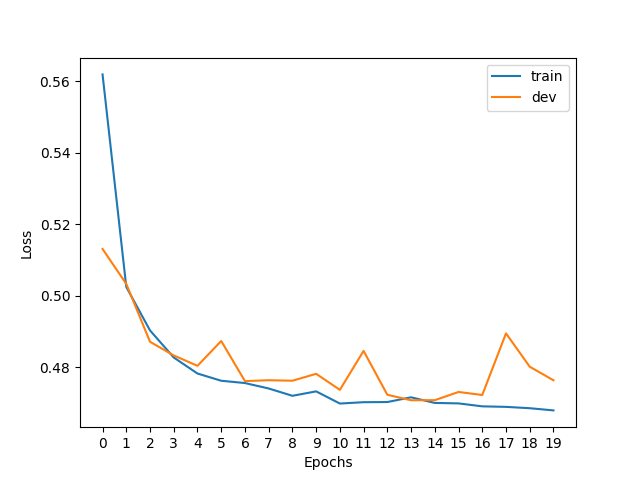
\includegraphics[width=0.48\textwidth]{hw3/mlp_none_loss.png}
  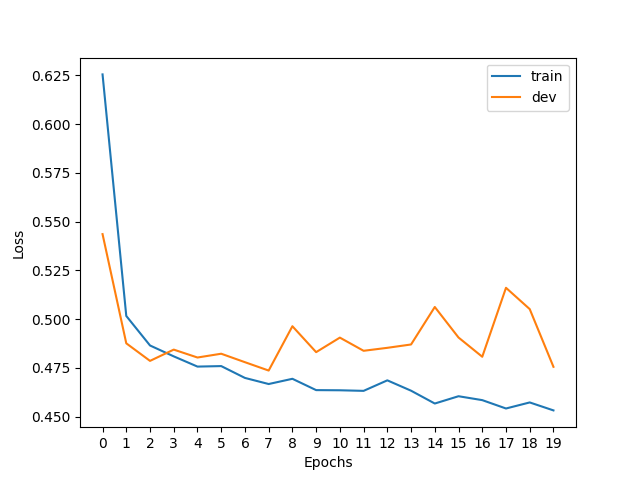
\includegraphics[width=0.48\textwidth]{hw3/mlp_512_loss.png}
\end{center}
\begin{center}
  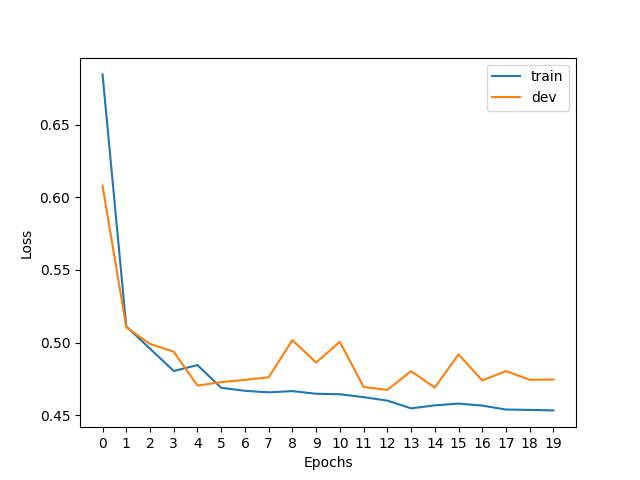
\includegraphics[width=0.48\textwidth]{hw3/mlp_512x512_loss.png}
  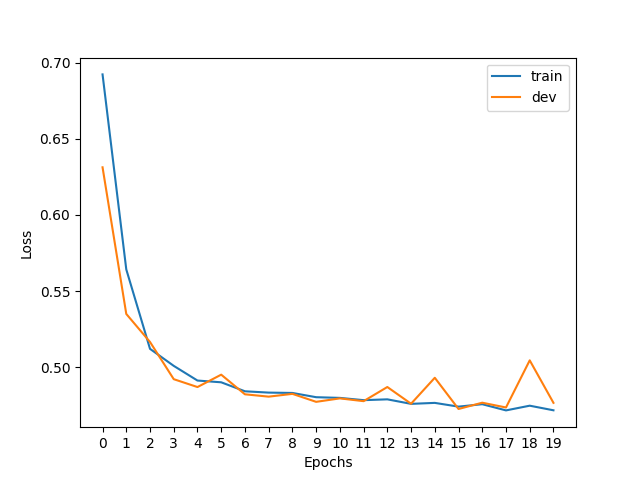
\includegraphics[width=0.48\textwidth]{hw3/mlp_512x512x512_loss.png}
\end{center}
\begin{center}
  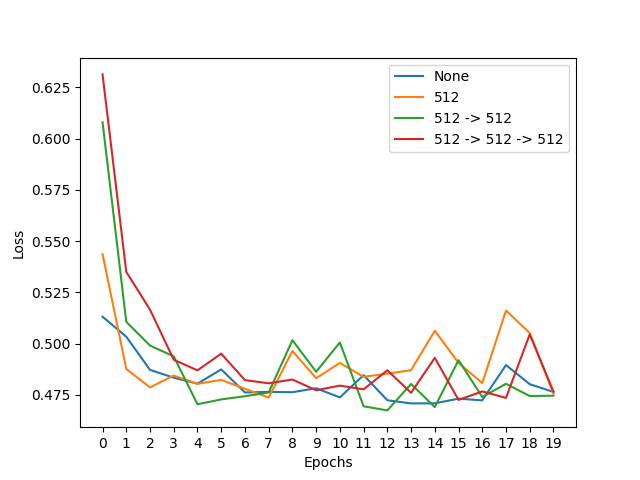
\includegraphics[width=0.48\textwidth]{hw3/all_mlp_loss.png}
  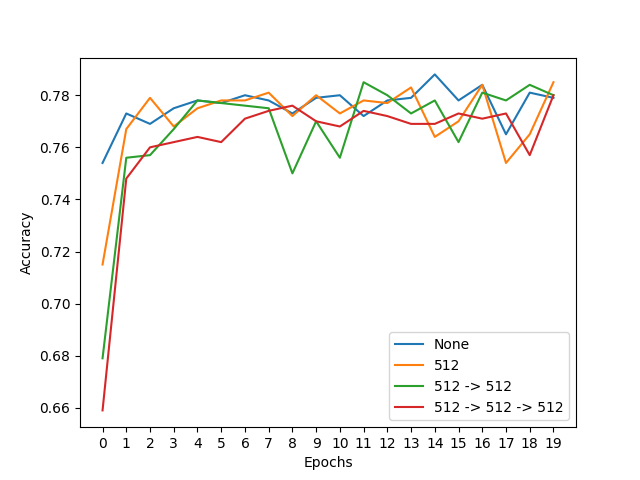
\includegraphics[width=0.48\textwidth]{hw3/all_mlp_acc.png}
\end{center}

\begin{center}
\small
\begin{tabular}{|l|r|r|r|r|}
  \hline
  Hidden layers & Parameters & Final dev loss & Best dev acc & Test acc \\
  \hline
  none (linear)         & 102     & 0.4764 & 0.7880 & 0.7800 \\
  512                   & 27{,}138  & 0.4756 & 0.7850 & 0.7910 \\
  512, 512              & 289{,}794 & 0.4746 & 0.7850 & 0.7810 \\
  512, 512, 512         & 552{,}450 & 0.4765 & 0.7800 & 0.7860 \\
  \hline
\end{tabular}
\end{center}

\textbf{Findings.}
All four architectures finish within 0.0019 of each other on final dev loss, 0.4746 to 0.4765, and within
0.008 on best dev accuracy, so depth buys nothing measurable on this task. What depth does change is the
start: initial dev loss rises monotonically with it, 0.5131, 0.5436, 0.6080 and 0.6313, so the deeper
models spend their early epochs catching up before converging to the same place. No dev curve ends more
than 0.0072 above its own minimum, so none of these models overfits; note too that this sweep varies
learning rate alongside depth (0.025, 0.02, 0.01, 0.001), so 6.1.5 is the controlled comparison.

\subsection*{6.1.4 Embrace Non-linearity: The Activation Functions}

\begin{center}
  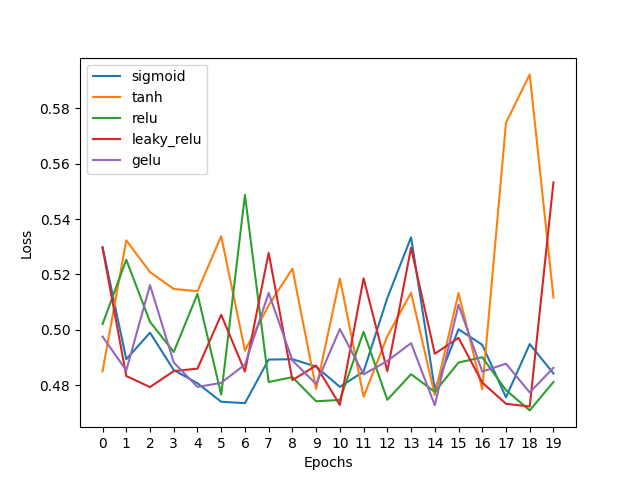
\includegraphics[width=0.48\textwidth]{hw3/mlp_activations_loss.png}
  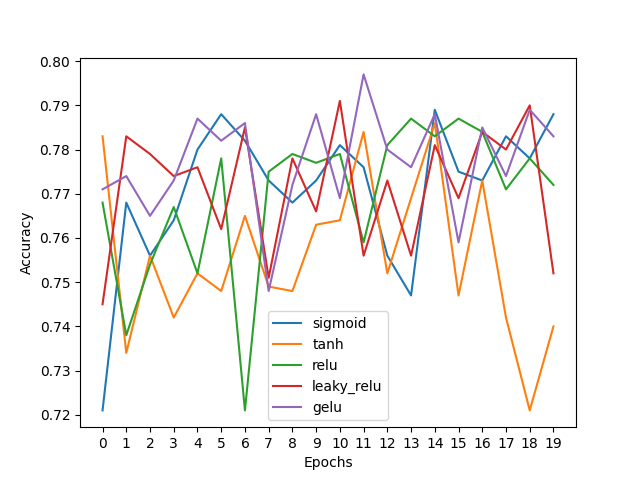
\includegraphics[width=0.48\textwidth]{hw3/mlp_activations_acc.png}
\end{center}

\begin{center}
\small
\begin{tabular}{|l|r|r|r|}
  \hline
  Activation & Final dev loss & Best dev acc & Test acc \\
  \hline
  \texttt{sigmoid}    & 0.4842 & 0.7890 & 0.7920 \\
  \texttt{tanh}       & 0.5117 & 0.7860 & 0.7860 \\
  \texttt{relu}       & 0.4812 & 0.7870 & 0.7740 \\
  \texttt{leaky\_relu} & 0.5533 & 0.7910 & 0.7900 \\
  \texttt{gelu}       & 0.4863 & 0.7970 & 0.7900 \\
  \hline
\end{tabular}
\end{center}

\textbf{Findings.}
Best dev accuracy spans only 0.011 across the five activations while final dev loss spans 0.0721, and that
gap is the finding: the loss spread reflects where each run landed on its last epoch, not the activation.
\texttt{leaky\_relu} sits at 0.4723 at epoch 18 and then jumps to 0.5533 at epoch 19, and \texttt{tanh}
oscillates between 0.4765 and 0.5922 over its last six epochs. I would not read this ordering as a ranking:
with one hidden layer there is a single activation derivative in the gradient path, so the saturation
differences separating sigmoid from ReLU never compound, and repeated seeds would be needed to rank them.

\subsection*{6.1.5 Hyper-parameter Tuning: Learning Rate}

\begin{center}
  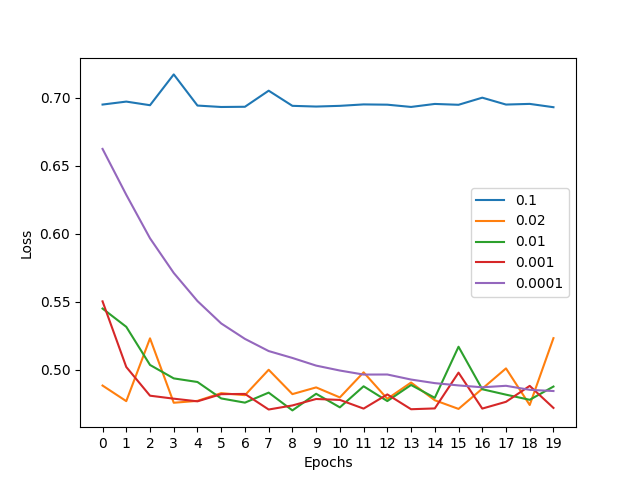
\includegraphics[width=0.48\textwidth]{hw3/mlp_learning_rates_loss.png}
  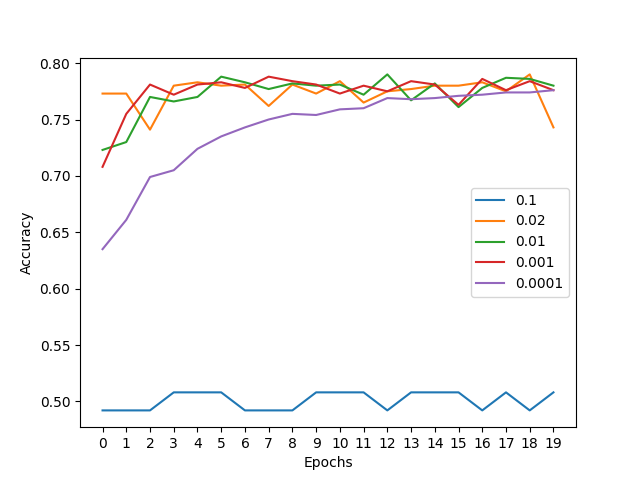
\includegraphics[width=0.48\textwidth]{hw3/mlp_learning_rates_acc.png}
\end{center}

\begin{center}
\small
\begin{tabular}{|l|r|r|r|}
  \hline
  Learning rate & Final dev loss & Best dev acc & Test acc \\
  \hline
  0.1    & 0.6929 & 0.5080 & 0.5010 \\
  0.02   & 0.5231 & 0.7900 & 0.7920 \\
  0.01   & 0.4875 & 0.7900 & 0.7810 \\
  0.001  & 0.4718 & 0.7880 & 0.7850 \\
  0.0001 & 0.4842 & 0.7760 & 0.7790 \\
  \hline
\end{tabular}
\end{center}

\textbf{Findings.}
At $\text{lr} = 0.1$ training fails outright: dev loss sits at 0.6929, essentially $\ln 2 = 0.6931$, dev
accuracy never leaves 0.492 or 0.508, and test accuracy is 0.501, so the model never improves on a constant
predictor. Below that the sweep is the expected U, falling to a minimum of 0.4718 at 0.001 and rising again
to 0.4842 at 0.0001, whose best epoch is its last and which therefore ran out of budget rather than became
unstable. Unlike 6.1.3 this experiment holds the architecture fixed at one 512-unit hidden layer with ReLU,
so learning rate is the only variable.

\end{document}
